\chapter{The Geometry of Homogeneous Space}

\lectureoverview{Flatness is an excellent approximation to the observed universe, but it is not a principle. If we retain homogeneity and isotropy while allowing curvature, three simply connected spatial geometries emerge: Euclidean, spherical, and hyperbolic space. Their metrics can be built from the way concentric shells grow with distance, and their curvature can be tested through angular sizes and object counts. Flat space may also be finite when its topology is toroidal. Finally, attaching a time-dependent scale factor to any of these homogeneous spaces gives the cosmological spacetime metrics and the Hubble law; dynamics for that scale factor must come from general relativity.}

\section{Flatness Is an Observation, Not a Principle}

Until now we have treated space as flat and have said almost nothing about spacetime geometry. Observation justifies flat space as a very good approximation, but it does not elevate flatness into a law. What the measurements really tell us is that any radius of curvature must be large compared with the region we have surveyed. Space might be exactly flat, positively curved, or negatively curved. On scales far beyond the observable region, we do not yet know which description is correct.

We therefore loosen one assumption while keeping another. We shall not assume flatness, but we shall continue to assume that space is homogeneous and isotropic. This is a working hypothesis, not an article of faith. To learn its consequences, we assume it and calculate; afterward we may abandon it and ask what an inhomogeneous universe would do differently.

Homogeneity means that every point has the same geometric character. An observer who moves elsewhere and repeats local geometric experiments obtains the same results. Isotropy means that no direction is preferred. These conditions exclude almost every curved surface one draws first. A paraboloid is more sharply curved near its tip than far from it. A long ellipsoid differs at its poles and waist. A bumped sphere, or the Earth's surface with mountains and valleys resolved, is curved but not homogeneous. The cosmological question is narrower:
\begin{quote}
Which spaces can be curved while still looking geometrically the same from every point and in every direction?
\end{quote}

Ignoring global identifications for the moment, there are three constant-curvature answers: flat space, positively curved spherical space, and negatively curved hyperbolic space. The qualification about global identifications matters; later we shall construct a flat finite torus and correct the oversimplified statement that these three exhaust every possibility.

\section{The Metric and the Observer's Coordinates}

We first discuss space alone, not spacetime. Its geometry is encoded in a metric: a rule for the squared distance \(ds^2\) between neighboring points. Once that local rule is known everywhere, lengths, angles, areas, volumes, geodesics, and curvature can all be recovered from it.

For a Euclidean plane and Euclidean three-space, Cartesian coordinates give
\begin{equation}
ds_2^2=dx^2+dy^2,
\qquad
ds_3^2=dx^2+dy^2+dz^2.
\label{eq:c03-cartesian-flat}
\end{equation}
Adding the third dimension simply adds the orthogonal term \(dz^2\), but the important point is not the simplicity of this formula. It is that equation~\eqref{eq:c03-cartesian-flat} completely specifies the local geometry.

\begin{figure}[htbp]
\centering

\includegraphics[width=0.74\textwidth]{lecture_03_figure_02.png}
\caption{The Cartesian metric of flat three-dimensional space, as written on the board.}
\label{fig:c03-cartesian-board}
\lectureframe{00:05:13.138}
\end{figure}

Cartesian coordinates conceal the way an astronomer encounters the universe. We occupy one point, look outward by direction, and sort what we see by angle and distance. In a two-dimensional universe the visual field would literally be a circle of directions around us. Polar coordinates are therefore not merely elegant; they expose the angular geometry that cosmology uses.

Let \(r\) be radial distance and \(\theta\) the direction. The same Euclidean plane now has metric
\begin{equation}
ds^2 = dr^2 + r^2 d\theta^2.
\label{eq:c03-polar-flat}
\end{equation}
For a fixed small angle \(d\theta\), the transverse separation is \(r\,d\theta\). It grows linearly as we move outward, and its squared contribution to the metric is consequently \(r^2d\theta^2\).

The angular term is itself the metric of a one-dimensional space. A circle is a one-sphere, denoted \(S^1\), and the metric of the unit circle is conventionally written
\begin{equation}
d\Omega_1^2 = d\theta^2,
\qquad\text{so that}\qquad
ds^2 = dr^2 + r^2 d\Omega_1^2.
\label{eq:c03-omega-one}
\end{equation}
The board uses \(d\Omega^2\) without a legible subscript; the spoken definition fixes the intended object as \(d\Omega_1^2\).

\begin{figure}[htbp]
\centering

\includegraphics[width=0.74\textwidth]{lecture_03_figure_03.png}
\caption{The polar-coordinate sketch and metric of flat space. The board shows \(d\Omega^2\); the explanation identifies it as the unit-circle metric \(d\Omega_1^2=d\theta^2\).}
\label{fig:c03-polar-board}
\lectureframe{00:08:37.254}
\end{figure}

\begin{figure}[htbp]
\centering
\begin{tikzpicture}[scale=1.2]
\draw[->] (-1.2,0)--(1.8,0);
\draw[->] (0,-1.2)--(0,1.8);
\draw[thick] (0,0)--(1.3,1.1);
\draw (0.7,0.7) node[above] {$r$};
\draw (0.58,0) arc (0:40:0.58);
\draw (0.8,0.22) node {$\theta$};
\end{tikzpicture}
\caption{A clean reconstruction of the observer-centered polar coordinates used in equation~\eqref{eq:c03-omega-one}.}
\label{fig:c03-polar-redraw}
\end{figure}

\begin{classroomqa}
\audiencequestion{Does \(d\theta^2\) really measure distance along the circumference?}
\lecturerresponse{Yes. On a unit circle, arc length equals angle in radians, so neighboring points separated by \(d\theta\) have squared intrinsic separation \(d\theta^2\). The circle has circumference \(2\pi\), and integrating \(ds=d\theta\) once around it gives precisely \(2\pi\). Multiplying by \(r^2\) enlarges the unit circle to the shell of radius \(r\) in the plane. \lecturetimestamp{00:09:11--00:09:26}}
\end{classroomqa}

The word \emph{intrinsic} is essential. If we embed the unit circle in a Euclidean plane, we may describe it by
\begin{equation}
x^2 + y^2 = 1.
\end{equation}
That equation describes how the circle sits in a larger space. It is not needed by an inhabitant who can measure only distances along the circle. We could bend a flexible optical fiber into a lopsided closed loop without stretching it. Its appearance in the plane would change, but its intrinsic circumference and its metric would not. Equal increments of \(\theta\) would still mark equal distances along the fiber. Geometry must therefore be separated from the accidental shape supplied by an embedding.

\begin{figure}[htbp]
\centering

\includegraphics[width=0.64\textwidth]{lecture_03_figure_04.png}
\caption{The board compares a round unit circle with a deformed closed loop. If the loop is bent without stretching, the two have the same intrinsic one-dimensional metric.}
\label{fig:c03-intrinsic-board}
\lectureframe{00:10:34.205}
\end{figure}

\begin{figure}[htbp]
\centering
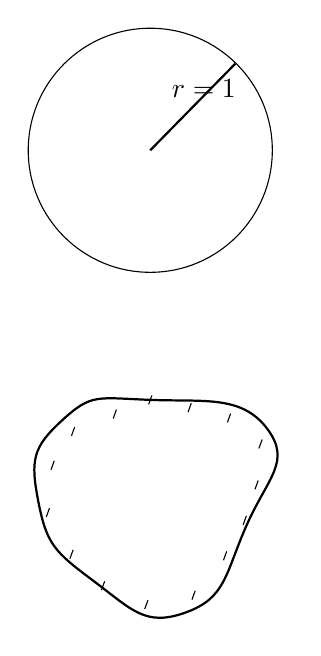
\begin{tikzpicture}[scale=1.0]
\draw (0,0) circle (1.55);
\draw[thick] (0,0)--(1.08,1.1);
\draw (0.68,0.78) node {$r=1$};

\begin{scope}[yshift=-4.35cm]
\draw[thick]
plot[smooth cycle, tension=0.95] coordinates
{(0,1.18) (1.48,0.82) (1.22,-0.42) (0.45,-1.52) (-0.72,-1.12) (-1.42,-0.12) (-1.12,0.92)};
\foreach \p in {(0,1.18),(0.5,1.08),(1.0,0.95),(1.4,0.62),(1.35,0.1),(1.2,-0.35),(0.95,-0.8),(0.55,-1.3),(-0.05,-1.42),(-0.6,-1.18),(-1.0,-0.78),(-1.3,-0.25),(-1.24,0.35),(-0.98,0.78),(-0.45,1.0)}{
\draw[rotate around={70:\p}] \p ++(-0.06,0) -- ++(0.12,0);
}
\end{scope}
\end{tikzpicture}
\caption{Intrinsic distance survives an extrinsic deformation: a one-dimensional inhabitant measures the same circumference in either embedding.}
\label{fig:c03-intrinsic-redraw}
\end{figure}

Flat space can now be read as a nested family of circles around the observer. The shell at distance \(r\) is a copy of the unit circle enlarged by \(r\), which is exactly what the factor \(r^2d\Omega_1^2\) records.

\section{Positive Curvature: Shells That Close}

A sphere is curved but homogeneous: no point on a perfectly round sphere is geometrically distinguished from another. We can build its metric without appealing to an external three-dimensional picture. Imagine two-dimensional astronomers who live on a unit \(2\)-sphere and place the origin of their coordinates at their own location.

The circle at a small geodesic distance \(r\) around them is small. As \(r\) increases, the circles grow, reach their greatest circumference halfway around the sphere, and then shrink until they collapse at the antipodal point. This growth and contraction occur with \emph{distance}, not with time. The sphere is static throughout this construction.

Here \(r\) is angular distance along the unit sphere rather than Euclidean distance from a center:
\[
0 \le r \le \pi.
\]
At \(r=0\) lies the chosen origin, at \(r=\pi/2\) the great circle halfway around, and at \(r=\pi\) the antipode. The radius of the shell is now \(\sin r\), so the flat factor \(r^2\) is replaced by \(\sin^2r\):
\begin{equation}
d\Omega_2^2 = dr^2 + \sin^2 r\, d\Omega_1^2
            = dr^2 + \sin^2 r\, d\theta^2.
\label{eq:c03-two-sphere}
\end{equation}
The endpoints and midpoint behave exactly as required:
\begin{equation}
\sin 0=0,
\qquad
\sin\frac{\pi}{2}=1,
\qquad
\sin\pi=0.
\end{equation}
Thus the shells begin at zero size, attain their maximum size, and close again.

\begin{figure}[htbp]
\centering

\includegraphics[width=0.82\textwidth]{lecture_03_figure_05.png}
\caption{The transition from nested circles in flat space to shells on the sphere. The lower formula is partly obscured in the frame; its spoken derivation gives the replacement \(r^2\mapsto\sin^2r\) in equation~\eqref{eq:c03-two-sphere}.}
\label{fig:c03-spherical-board}
\lectureframe{00:16:11.701}
\end{figure}

\begin{figure}[htbp]
\centering
\resizebox{\linewidth}{!}{%
\begin{tikzpicture}[scale=0.92]
\begin{scope}[xshift=-4.15cm]
\draw[->] (-1.7,0)--(1.9,0);
\draw[->] (0,-1.7)--(0,1.9);
\draw (0,0) circle (0.45);
\draw (0,0) circle (0.9);
\draw (0,0) circle (1.35);
\draw[thick] (0,0)--(1.45,1.2);
\draw (0.56,0.18) arc (18:40:0.63);
\draw (0.94,0.44) node {$\theta$};
\end{scope}

\begin{scope}[xshift=4.15cm]
\draw (0,0) circle (2.0);
\fill (0,-2.0) circle (1.5pt);
\fill (2.0,0) circle (1.5pt);
\fill (0,2.0) circle (1.5pt);
\draw[thick] (0,-2.0) arc (-90:90:2.0);
\draw (0,-2.35) node {$r=0$};
\draw (2.75,0) node {$r=\pi/2$};
\draw (0,2.35) node {$r=\pi$};
\end{scope}
\end{tikzpicture}
}%
\caption{Flat shells grow forever, whereas spherical shells grow to a maximum at \(r=\pi/2\) and close at \(r=\pi\).}
\label{fig:c03-shells-flat-sphere}
\end{figure}

The notation \(d\Omega_2^2\) means the metric of the unit \(2\)-sphere, just as \(d\Omega_1^2\) means the metric of its circular shells. The same recursive construction works one dimension higher. At fixed radius in flat three-space, the shell around us is a \(2\)-sphere:
\begin{equation}
ds_{\text{flat},3}^2 = dr^2 + r^2 d\Omega_2^2.
\label{eq:c03-flat-three-polar}
\end{equation}
If those \(2\)-sphere shells grow and then close with the factor \(\sin r\), the resulting space is a unit \(3\)-sphere:
\begin{equation}
d\Omega_3^2 = dr^2 + \sin^2 r\, d\Omega_2^2.
\label{eq:c03-three-sphere}
\end{equation}
The \(3\)-sphere is difficult to picture because its familiar embedding would require four Euclidean dimensions. The metric, however, is complete and needs no picture. Around any chosen observer sit nested \(2\)-spheres; they grow to a maximum and then shrink to the antipodal point.

\begin{classroomqa}
\audiencequestion{Is the observer at the center of the sphere?}
\lecturerresponse{The observer is at the center of the \emph{coordinate shells}, not at a privileged geometric center. The origin is a point on the space, and any other observer may choose their own point as \(r=0\) and obtain the same metric. Homogeneity is precisely the statement that no such choice is preferred. \lecturetimestamp{00:19:21--00:20:27}}
\end{classroomqa}

For visualization alone, the unit circle and the unit \(2\)-sphere can be embedded in Euclidean spaces:
\begin{equation}
x^2+y^2=1,
\qquad
x^2+y^2+z^2=1.
\end{equation}
These equations describe embeddings, not extra physics. An ant confined to the circle or sphere can determine the intrinsic metric without detecting the surrounding Euclidean space. Likewise, \(S^3\) is not an ordinary ball with a mysterious boundary. It is the complete three-dimensional space described by equation~\eqref{eq:c03-three-sphere}.

\section{How Curvature Changes What We See}

Geometry becomes physics only when it changes an observation. Suppose an object has known transverse diameter \(d\), its radial distance \(r\) has been inferred independently, and its angular diameter \(d\theta\) is measured on the sky. Galaxies provide a rough intuitive example; more precise cosmology uses calibrated standard rulers and standard candles. Distance information can be assembled from spectral redshift, the Hubble relation, luminosity, and cross-calibration among different classes of objects.

In flat space, hold \(r\) fixed across the transverse width of the object. Equation~\eqref{eq:c03-polar-flat} gives
\begin{equation}
d^2 = r^2 d\theta^2.
\label{eq:c03-flat-angle-step}
\end{equation}
Therefore
\begin{equation}
d\theta = \frac{d}{r}.
\label{eq:c03-flat-angle}
\end{equation}
Angular size falls inversely with distance.

On a unit sphere, the transverse shell size is \(\sin r\) rather than \(r\):
\begin{equation}
d^2 = \sin^2 r\, d\theta^2,
\qquad\text{hence}\qquad
d\theta = \frac{d}{\sin r}.
\label{eq:c03-spherical-angle}
\end{equation}
For \(0<r<\pi\), \(\sin r<r\), so the same object at the same radial distance looks larger than it would in flat space. Its angular size first decreases, reaches a minimum at the equator, and then increases as the shell contracts. In the limiting idealization at the antipode, all directions meet and the image spreads around the sky.

\begin{classroomqa}
\audiencequestion{Is this the same idea used to infer curvature from the cosmic microwave background?}
\lecturerresponse{Yes. The early plasma supplies a characteristic physical scale through its acoustic oscillations. We measure the angle subtended by that standard ruler and compare it with the angle predicted by each geometry. The objects need not literally be galaxies; the essential comparison is a known transverse scale against its observed angular size. \lecturetimestamp{00:37:37--00:38:12}}
\end{classroomqa}

Shell volumes provide a second test. In three flat dimensions, the area of a shell is proportional to \(r^2\); on a unit \(3\)-sphere it is proportional to \(\sin^2r\). A homogeneous population therefore first becomes more numerous with distance on a spherical shell and then less numerous after the equator. Positive curvature predicts a paired signature relative to flat space: sufficiently distant standard rulers look too large, and sufficiently distant shells contain too few objects.

\begin{figure}[htbp]
\centering
\resizebox{\linewidth}{!}{%
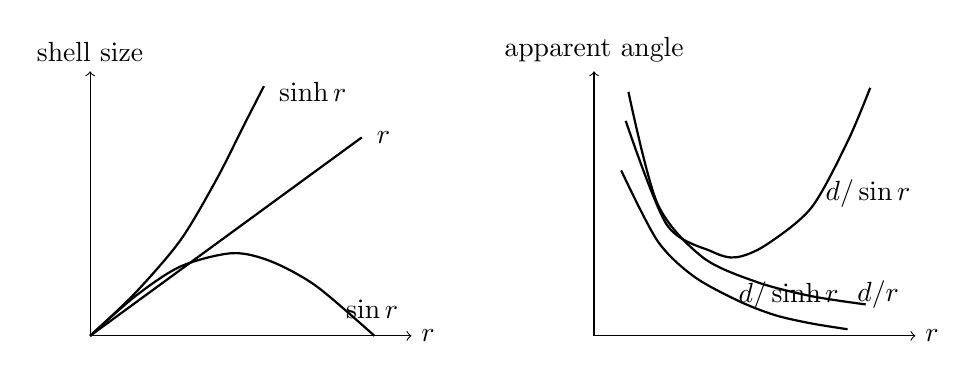
\begin{tikzpicture}[x=1.15cm,y=1.05cm]
\begin{scope}
\draw[->] (0,0)--(3.55,0) node[right] {$r$};
\draw[->] (0,0)--(0,3.2) node[above] {shell size};

\draw[thick] (0,0)--(3.0,2.4);
\draw (3.06,2.4) node[right] {$r$};

\draw[thick]
plot[smooth] coordinates {(0,0) (0.5,0.48) (1.0,0.84) (1.57,1.0) (2.0,0.9) (2.5,0.6) (3.14,0)};
\draw (2.72,0.55) node[below right] {$\sin r$};

\draw[thick]
plot[smooth] coordinates {(0,0) (0.5,0.52) (1.0,1.16) (1.4,1.9) (1.7,2.55) (1.92,3.02)};
\draw (1.98,2.95) node[right] {$\sinh r$};
\end{scope}

\begin{scope}[xshift=6.4cm]
\draw[->] (0,0)--(3.55,0) node[right] {$r$};
\draw[->] (0,0)--(0,3.2) node[above] {apparent angle};

\draw[thick]
plot[smooth] coordinates {(0.38,2.95) (0.7,1.6) (1.2,0.95) (1.8,0.65) (2.4,0.48) (3.0,0.38)};
\draw (2.8,0.5) node[right] {$d/r$};

\draw[thick]
plot[smooth] coordinates {(0.35,2.6) (0.8,1.35) (1.3,1.02) (1.57,0.95) (1.9,1.1) (2.4,1.55) (2.8,2.35) (3.05,3.0)};
\draw (2.45,1.72) node[right] {$d/\sin r$};

\draw[thick]
plot[smooth] coordinates {(0.3,2.0) (0.7,1.15) (1.1,0.72) (1.6,0.42) (2.0,0.25) (2.4,0.15) (2.8,0.08)};
\draw (2.15,0.2) node[above] {$d/\sinh r$};
\end{scope}
\end{tikzpicture}
}%
\caption{The radial shell factors and corresponding angular-size laws. Positive curvature makes the shell close; negative curvature makes it grow exponentially.}
\label{fig:c03-shell-angular-laws}
\end{figure}

\begin{classroomqa}
\audiencequestion{Does the radial coordinate become infinite as we continue around the sphere?}
\lecturerresponse{No. On the unit sphere, \(r\) is geodesic angular distance and ranges only from \(0\) to \(\pi\). At \(r=\pi\) the shell has collapsed at the antipode. We are examining a fixed spatial geometry here, not following an object outward through time. Introducing a curvature radius later multiplies all physical distances by that radius but does not change this dimensionless range. \lecturetimestamp{00:39:30--00:40:35}}
\end{classroomqa}

\section{Projection Is Not Geometry}

Before turning to negative curvature, it is useful to see how badly a faithful geometry can be distorted by a picture. Rest a sphere on a plane tangent at its south pole. Draw a line from the north pole through each point \(P\) on the sphere and continue it to the plane at \(P'\). This is stereographic projection. The north pole itself is sent to infinity. A small region near the south pole is represented with little distortion, whereas equal intrinsic regions near the north pole become enormous on the plane.

The distortion belongs to the map, not to the sphere. The source sphere remains homogeneous even though its planar image assigns wildly different coordinate sizes to equivalent regions. This discipline will be needed again when an infinite hyperbolic space is compressed into a finite disk.

\begin{figure}[htbp]
\centering
\resizebox{\linewidth}{!}{%
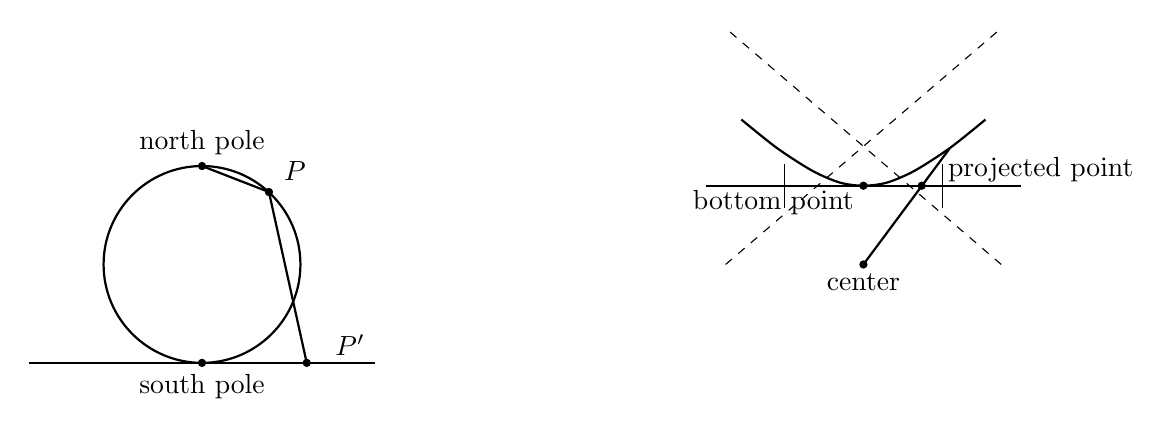
\begin{tikzpicture}[scale=1.0]
\begin{scope}[xshift=-4.2cm]
\draw[thick] (-2.2,-1.25)--(2.2,-1.25);
\draw[thick] (0,0) circle (1.25);
\fill (0,1.25) circle (1.5pt);
\fill (0,-1.25) circle (1.5pt);
\draw (0,1.55) node {north pole};
\draw (0,-1.55) node {south pole};

\fill (0.85,0.92) circle (1.5pt);
\draw (0.92,1.18) node[right] {$P$};
\draw[thick] (0,1.25)--(0.85,0.92)--(1.33,-1.25);
\fill (1.33,-1.25) circle (1.5pt);
\draw (1.57,-1.03) node[right] {$P'$};
\end{scope}

\begin{scope}[xshift=4.2cm]
\draw[thick] (-2.0,1)--(2.0,1);
\draw[dashed] (-1.75,0)--(1.75,3.0);
\draw[dashed] (1.75,0)--(-1.75,3.0);
\draw[thick]
plot[smooth] coordinates
{(-1.55,1.84) (-1.1,1.48) (-0.65,1.19) (-0.3,1.04) (0,1.0) (0.3,1.04) (0.65,1.19) (1.1,1.48) (1.55,1.84)};
\fill (0,0) circle (1.5pt);
\fill (0,1) circle (1.5pt);
\draw (0,-0.22) node {center};
\draw (0,0.78) node[left] {bottom point};
\draw[thick] (0,0)--(1.1,1.48);
\fill (0.74,1.0) circle (1.5pt);
\draw (0.95,1.2) node[right] {projected point};
\draw (-1,0.72) -- (-1,1.28);
\draw (1,0.72) -- (1,1.28);
\end{scope}
\end{tikzpicture}
}%
\caption{Left: stereographic projection sends the north pole of a sphere to infinity. Right: a hyperboloid can be projected into a finite disk, represented here by a cross-sectional interval. Coordinate distortion does not destroy intrinsic homogeneity.}
\label{fig:c03-projections}
\end{figure}

\section{Negative Curvature: Shells That Outgrow Flat Space}

The third simply connected homogeneous geometry replaces \(\sin r\) by the hyperbolic sine. Its unit metrics in two and three dimensions are
\begin{equation}
dh_2^2 = dr^2 + \sinh^2 r\, d\Omega_1^2,
\label{eq:c03-hyperbolic-two}
\end{equation}
\begin{equation}
dh_3^2 = dr^2 + \sinh^2 r\, d\Omega_2^2.
\label{eq:c03-hyperbolic-three}
\end{equation}
The coordinate \(r\) now ranges over
\begin{equation}
0\le r<\infty.
\end{equation}
Near the origin, \(\sinh r\approx r\), so the geometry is locally Euclidean. Far away, its shells grow much faster than Euclidean shells and never turn around.

The growth law follows from
\begin{equation}
\sin r = \frac{e^{ir}-e^{-ir}}{2i},
\qquad
\sinh r = \frac{e^r-e^{-r}}{2}.
\label{eq:c03-sin-sinh}
\end{equation}
At large \(r\), \(\sinh r\sim e^r/2\). In two dimensions, circumference therefore grows exponentially with radius; in three dimensions, shell area grows as \(\sinh^2r\sim e^{2r}/4\). A homogeneous distribution contains correspondingly many objects on a distant shell.

For a transverse object of size \(d\),
\begin{equation}
d^2 = \sinh^2 r\, d\theta^2,
\qquad\text{so}\qquad
d\theta = \frac{d}{\sinh r}.
\label{eq:c03-hyperbolic-angle}
\end{equation}
At large \(r\),
\begin{equation}
d\theta \sim 2d\,e^{-r}.
\end{equation}
Negative curvature therefore gives the opposite signature from positive curvature: distant standard rulers look too small, while distant shells contain too many objects relative to flat space.

\begin{classroomqa}
\audiencequestion{How do the radial ranges distinguish spherical and hyperbolic space?}
\lecturerresponse{On the unit sphere, \(r\) stops at the antipode, \(r=\pi\). In hyperbolic space it continues without bound, \(0\le r<\infty\). The shell factor reveals the same contrast: \(\sin r\) returns to zero, whereas \(\sinh r\) increases forever. \lecturetimestamp{00:52:46--00:53:25}}
\end{classroomqa}

There is an embedding that makes homogeneity less mysterious. Introduce ambient coordinates \(T,x,y\), where \(T\) is only an embedding coordinate and is \emph{not} cosmological time, and take the upper sheet
\begin{equation}
T^2 - x^2 - y^2 = 1.
\label{eq:c03-hyperboloid}
\end{equation}
Equip the ambient space with the Lorentz-signature metric
\begin{equation}
d\ell_{\mathrm{emb}}^2=-dT^2+dx^2+dy^2.
\label{eq:c03-ambient-minkowski}
\end{equation}
The metric induced on the hyperboloid is positive definite. Lorentz transformations preserve both equations~\eqref{eq:c03-hyperboloid} and~\eqref{eq:c03-ambient-minkowski}, and they can move any point of the upper sheet to any other. In that sense, changing the origin on hyperbolic space is like tilting the time axis in the auxiliary ambient space. Every point is geometrically equivalent.

Project the hyperboloid into a disk and infinitely distant points accumulate at the boundary circle. Nearby regions are drawn nearly faithfully; regions farther away are compressed ever more strongly. This is the Poincar\'e disk representation familiar from repeating figures of angels and devils. A coordinate transformation can move an apparently tiny figure near the edge to the center, where it becomes large, while preserving all intrinsic lengths and angles. In three dimensions the corresponding model is a ball rather than a disk. The names \emph{Poincar\'e space}, \emph{Lobachevsky space}, and \emph{space of uniform negative curvature} refer to this same local geometry.

\begin{classroomqa}
\audiencequestion{Is the finite disk like a Penrose diagram?}
\lecturerresponse{It is similar in the limited sense that an infinite domain is represented inside a finite picture. Here, however, the disk represents space alone, not spacetime or causal infinity. Its boundary is infinitely far away in the intrinsic hyperbolic metric even though the drawing places it at a finite coordinate radius. \lecturetimestamp{01:02:55--01:03:05}}
\end{classroomqa}

\section{The Radius of Curvature}

The metrics written so far describe unit geometries. To give a sphere or hyperbolic space an arbitrary curvature radius, multiply every length by a constant. The board denotes that constant by \(a\); to avoid confusing it with the time-dependent cosmological scale factor used later, we shall call the static curvature radius \(R_c\). Since the metric measures squared length,
\begin{align}
ds_{\mathrm{sph}}^2
  &=R_c^2d\Omega_n^2
   =R_c^2\left(dr^2+\sin^2r\,d\Omega_{n-1}^2\right),\\
ds_{\mathrm{hyp}}^2
  &=R_c^2dh_n^2
   =R_c^2\left(dr^2+\sinh^2r\,d\Omega_{n-1}^2\right).
\label{eq:c03-scaled-curvature}
\end{align}
The physical radial distance is \(R_cr\). Enlarging \(R_c\) makes the space less curved; the magnitude of constant sectional curvature scales as \(1/R_c^2\). In the limit \(R_c\to\infty\), both curved metrics approach Euclidean geometry on every fixed finite region.

\begin{classroomqa}
\audiencequestion{If the sphere is made twice as large, does it become more curved or less curved?}
\lecturerresponse{Less curved. The first answer offered in class was corrected by comparing a basketball with Earth: the smaller surface bends more rapidly over a given distance. Doubling \(R_c\) halves the inverse-radius curvature scale and divides sectional curvature \(1/R_c^2\) by four. \lecturetimestamp{01:10:14--01:10:56}}
\end{classroomqa}

This explains why all three geometries look alike nearby. For \(r\ll1\),
\begin{equation}
\sin r=r-\frac{r^3}{6}+\cdots,
\qquad
\sinh r=r+\frac{r^3}{6}+\cdots.
\end{equation}
The leading term in either curved metric is the flat polar metric; curvature first appears through corrections of relative order \((L/R_c)^2\) across a physical scale \(L\).

\begin{classroomqa}
\audiencequestion{Do observations tell us whether space is flat, spherical, or hyperbolic?}
\lecturerresponse{They tell us that the observable region is very close to flat. The rough classroom estimate was that a one-percent bound on curvature effects implies \(R_c\) at least about ten times the size of the visible region, because \((L/R_c)^2\lesssim10^{-2}\). A corresponding curvature volume would then be at least roughly \(10^3\) visible volumes. This is an order-of-magnitude lecture estimate, not a current precision-data quotation, and exact flatness remains the \(R_c=\infty\) possibility. \lecturetimestamp{01:11:00--01:13:37}}
\end{classroomqa}

\section{Flat but Finite: The Torus}

We must now correct the statement that flat, spherical, and hyperbolic spaces are the only homogeneous possibilities. They are the three simply connected constant-curvature geometries. A flat space can also have nontrivial global topology.

Begin with a Euclidean rectangle. Identify its left edge point by point with its right edge, and identify its bottom edge with its top. Crossing any edge returns through the opposite one. The local metric remains \(dx^2+dy^2\), but the global space is periodic and finite. This quotient is a flat two-torus \(T^2\). One periodic dimension gives a circle \(T^1\), identifying opposite faces of a rectangular box gives a flat three-torus \(T^3\), and the construction extends to any number of dimensions.

\begin{figure}[htbp]
\centering
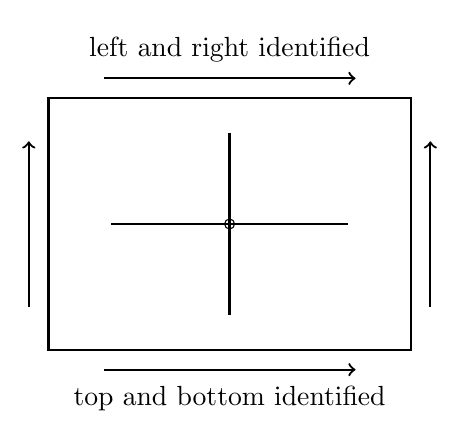
\begin{tikzpicture}[scale=1.0]
\draw[thick] (0,0) rectangle (4.6,3.2);

\draw[->,thick] (0.7,3.45)--(3.9,3.45);
\draw[->,thick] (0.7,-0.25)--(3.9,-0.25);

\draw[->,thick] (-0.25,0.55)--(-0.25,2.65);
\draw[->,thick] (4.85,0.55)--(4.85,2.65);

\draw[thick] (0.8,1.6)--(3.8,1.6);
\draw[thick] (2.3,0.45)--(2.3,2.75);

\draw (2.3,1.6) circle (1.8pt);

\draw (2.3,-0.62) node {top and bottom identified};
\draw (2.3,3.82) node {left and right identified};
\end{tikzpicture}
\caption{A flat torus constructed by identifying opposite sides of a rectangle. The edges are not boundaries; paired points are the same points of the quotient space.}
\label{fig:c03-flat-torus}
\end{figure}

\begin{classroomqa}
\audiencequestion{Can a universe therefore be both flat and finite?}
\lecturerresponse{Yes. Flatness is a local statement about the metric; finiteness can be a global statement about topology. A sufficiently large three-torus would look Euclidean throughout the region we can observe even though its total volume is finite. \lecturetimestamp{01:13:37--01:17:59}}
\end{classroomqa}

The universal-cover picture makes the observable consequence transparent. Instead of identifying the edges, tile an infinite Euclidean plane with copies of the fundamental rectangle. A single object in the torus appears once in every copy. In three dimensions the copies form a periodic crystal-like array.

\begin{classroomqa}
\audiencequestion{Could we live in a toroidal universe without noticing it?}
\lecturerresponse{Yes, if the fundamental cell is larger than the region from which light has reached us. If it were small enough, light could traverse the identifications and we would see repeated images of the same galaxies, perhaps even repeated views of our own neighborhood, in different directions. The local geometry would remain flat in either case. \lecturetimestamp{01:18:16--01:22:04}}
\end{classroomqa}

\begin{classroomqa}
\audiencequestion{Why does the sphere stop at its antipode while the torus repeats?}
\lecturerresponse{On the sphere, the surrounding shell genuinely shrinks to zero at \(r=\pi\); all radial directions meet at the antipode. On a torus, the edge of a chosen rectangular cell never shrinks. It is identified with an equally large opposite edge, so crossing it continues the same space in a periodic coordinate description. \lecturetimestamp{01:22:06--01:23:02}}
\end{classroomqa}

\section{From Space to Spacetime}

We can now restore time. In units with the speed of light \(c=1\), the Minkowski metric is
\begin{equation}
ds^2 = -dt^2 + dx^2 + dy^2 + dz^2.
\label{eq:c03-minkowski}
\end{equation}
The sign convention is a choice; what matters is that the temporal term has the opposite sign from the spatial terms. A light ray follows a null trajectory,
\begin{equation}
ds^2 = 0.
\end{equation}
For motion only along \(x\),
\begin{equation}
-dt^2 + dx^2 = 0
\qquad\Rightarrow\qquad
dx = \pm dt.
\label{eq:c03-null-flat}
\end{equation}
The two signs describe light moving left or right at unit speed.

For cosmology, keep the proper-time term \(-dt^2\), replace the Euclidean spatial part by a homogeneous spatial metric, and let its overall scale vary with time. We denote this scale factor by \(a(t)\). It is now a dynamical function rather than the fixed radius \(R_c\) used in the static comparison.

As a pictureable \(2+1\)-dimensional example, take
\begin{equation}
ds^2 = -dt^2 + a(t)^2 d\Omega_2^2.
\label{eq:c03-two-plus-one}
\end{equation}
At each fixed \(t\), space is a \(2\)-sphere of radius \(a(t)\). Stacking these spheres in time gives the spacetime. The familiar \(3+1\)-dimensional construction is
\begin{equation}
ds^2 = -dt^2 + a(t)^2 d\Sigma^2,
\label{eq:c03-frw-general}
\end{equation}
where \(d\Sigma^2\) is a time-independent unit spatial metric. The three simply connected cases are
\begin{align}
\text{flat:}\quad
ds^2&=-dt^2+a(t)^2\left(dx^2+dy^2+dz^2\right),\label{eq:c03-frw-flat}\\
\text{spherical:}\quad
ds^2&=-dt^2+a(t)^2d\Omega_3^2,\label{eq:c03-frw-spherical}\\
\text{hyperbolic:}\quad
ds^2&=-dt^2+a(t)^2dh_3^2.\label{eq:c03-frw-hyperbolic}
\end{align}
The relative scale of comoving coordinates is fixed while \(a(t)\) changes. In the spherical and hyperbolic normalizations, \(a(t)\) is also the instantaneous curvature radius. In the flat case its absolute normalization can be absorbed into the comoving coordinates.

The Hubble law follows before any gravitational field equation is imposed. Consider two nearby comoving points with fixed coordinate separation \(\chi\). Their physical separation is
\begin{equation}
D(t)=a(t)\chi.
\label{eq:c03-comoving-distance}
\end{equation}
Differentiating at fixed \(\chi\) gives
\begin{equation}
V=\dot D=\dot a(t)\chi.
\end{equation}
Eliminating \(\chi\),
\begin{equation}
V = \frac{\dot a}{a} D.
\label{eq:c03-hubble-law}
\end{equation}
Thus
\begin{equation}
H = \frac{\dot a}{a}.
\label{eq:c03-hubble-parameter}
\end{equation}
This is a kinematic identity for homogeneous expansion or contraction. It holds for all three spatial geometries: \(\dot a>0\) gives recession, and \(\dot a<0\) gives approach.

Geometry alone does not determine \(a(t)\). Functions such as
\begin{equation}
a(t)\propto t^{2/3},
\qquad
a(t)\propto t^{1/2},
\qquad
a(t)\propto e^{Ht}
\end{equation}
all fit the homogeneous metric ansatz but describe different cosmic matter and energy contents. General relativity supplies the dynamical equation that selects among them. The resulting Friedmann equation will also connect the flat, spherical, and hyperbolic cases with the zero-, negative-, and positive-energy alternatives of the Newtonian cosmology developed earlier.

\begin{classroomqa}
\audiencequestion{Could the geometry and the cosmic evolution be much more complicated than these models?}
\lecturerresponse{Certainly. Homogeneity and isotropy are restrictive assumptions, chosen because they are natural, observationally successful on large scales, and mathematically tractable. Many more complicated geometries and evolutions exist. An important dynamical question is whether broad classes of initially irregular models evolve toward one of these simple homogeneous forms. \lecturetimestamp{01:36:00--01:36:50}}
\end{classroomqa}

\begin{classroomqa}
\audiencequestion{Is the \(3\)-sphere the boundary of a four-dimensional object?}
\lecturerresponse{It can be represented that way as an embedding, but the cosmological space is the \(3\)-sphere itself. It has three intrinsic dimensions and no boundary. The four-dimensional Euclidean picture is optional scaffolding; equation~\eqref{eq:c03-three-sphere} already defines the geometry completely. \lecturetimestamp{01:36:55--01:37:59}}
\end{classroomqa}

\begin{classroomqa}
\audiencequestion{Is luminosity the only way to obtain the distance needed for the curvature test?}
\lecturerresponse{No. Spectral lines identify redshift, nearby distance ladders calibrate the Hubble relation, and supernovae provide approximately standard luminosities. These methods are cross-checked rather than trusted in isolation. Even the inverse-square luminosity law depends on geometry because the area of a light front is set by \(r^2\), \(\sin^2r\), or \(\sinh^2r\). The agreement of several observables is what supports near-flatness. \lecturetimestamp{01:38:00--01:41:07}}
\end{classroomqa}

\section{What to Carry Forward}

The geometry of a homogeneous universe can be read from the growth of shells around any observer:
\begin{equation}
f(r)=
\begin{cases}
r, & \text{flat space},\\
\sin r, & \text{positive curvature},\\
\sinh r, & \text{negative curvature}.
\end{cases}
\end{equation}
The spatial metric is \(dr^2+f(r)^2d\Omega_{n-1}^2\). The same function controls angular sizes and the number of objects available on a shell, so curvature has direct observational meaning. A large curvature radius hides these differences locally, and a toroidal identification shows that local curvature does not by itself determine global size or topology.

Adding \(-dt^2\) and the common factor \(a(t)^2\) turns any of the three homogeneous spatial metrics into a cosmological spacetime. It immediately yields \(V=HD\) with \(H=\dot a/a\), but it leaves \(a(t)\) undetermined. The next step is therefore not another exercise in geometry. It is the dynamical problem: use Einstein's equations to determine how matter, radiation, curvature, and other forms of energy make the scale factor evolve.
